\documentclass{standalone}

\usepackage{pgfplots}
\pgfplotsset{compat=1.10}   % in my packages used compat=1.15
\usepgfplotslibrary{fillbetween}
\usepackage{pgf}
\usepackage{tikz}
\usetikzlibrary{patterns,arrows,calc,decorations.pathmorphing,backgrounds, positioning,fit,petri,decorations.fractals}
\usetikzlibrary{matrix}

\usepackage[table,dvipsnames]{tudscrcolor}

\usepackage[default]{opensans}

\begin{document}
	\color{cddarkblue}
	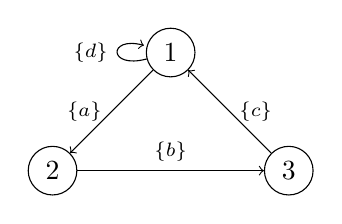
\begin{tikzpicture}[auto]
	% Knoten
		\node (1) at (0,0)  [circle,draw] {1};
		\node (2) at (-1.5,-1.5) [circle,draw] {2};
		\node (3) at (1.5,-1.5) [circle,draw] {3};
	% Kanten
%		\path (1) -> node[weight] {$3$} (3)
		\draw[->, loop left]  (1) edge node[left]{\scriptsize $\{ d \}$} (1);
		\draw[->]  (1) edge node[left]{\scriptsize $\{ a \}$} (2);
		\draw[->] (2) edge node{\scriptsize $\{ b \}$} (3);
		\draw[->] (3) edge node[right]{\scriptsize $\{ c \}$} (1);
	\end{tikzpicture}
\end{document}